\documentclass[border=5pt]{standalone}
\usepackage[utf8]{inputenc}
\usepackage{amssymb}
\usepackage{amsmath}
\usepackage{tikz}
\usetikzlibrary{arrows.meta}

\begin{document}
\nopagecolor
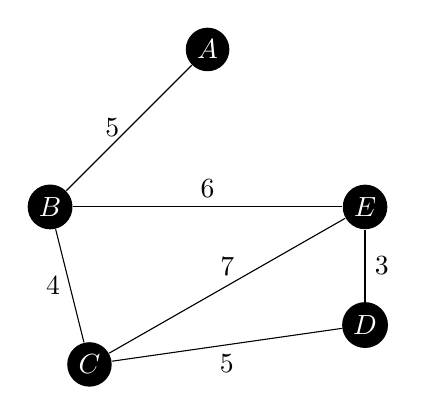
\begin{tikzpicture}
    \node[circle, inner sep=2pt, fill] (a) at (0, 0) {\color{white} $A$};
    \node[circle, inner sep=2pt, fill] (b) at (-2, -2) {\color{white} $B$};
    \node[circle, inner sep=2pt, fill] (c) at (-1.5, -4) {\color{white} $C$};
    \node[circle, inner sep=2pt, fill] (d) at (2, -3.5) {\color{white} $D$};
    \node[circle, inner sep=2pt, fill] (e) at (2, -2) {\color{white} $E$};

    \draw (a) edge[left] node{5} (b)
          (b) edge[left] node{4} (c)
          (b) edge[above] node{6} (e)
          (c) edge[above] node{7} (e)
          (c) edge[below] node{5} (d)
          (d) edge[right] node{3} (e);
\end{tikzpicture}
\end{document}